\documentclass{beamer}
\usepackage[utf8]{inputenc}
\usepackage{amsmath}
%\usepackage{algorithm}
%\usepackage{algorithmic}
\usepackage{graphicx}
\usepackage{lipsum}
\usepackage[linesnumbered,ruled,vlined]{algorithm2e}
% Tema da apresentação
\usetheme{CambridgeUS}
\usepackage{tikz}
\usetikzlibrary{shapes.geometric, arrows, backgrounds, calc}
\usetikzlibrary{shapes, positioning, circuits.ee.IEC}
\usepackage{qrcode}


% Pacote de cores
\usecolortheme{seahorse}

%------------------------------------------------------------
%\titlegraphic{\includegraphics[height=1.4cm]{Image/UFRPE.jpg}
%\hfill
%\raisebox{.3\height}{\includegraphics[height=0.8cm]{Image/ppgg.png}}
% }

 
% Definir paleta de cores
\definecolor{techblue}{RGB}{0, 102, 204}
\definecolor{techgreen}{RGB}{34, 153, 84}
\definecolor{techgray}{RGB}{240, 240, 240}
\definecolor{codebg}{RGB}{30, 30, 30}
\definecolor{techred}{RGB}{204, 0, 0} % Adicionado
\definecolor{techyellow}{RGB}{204, 204, 0} % Adicionado

% Personalizar estilo dos títulos e subtítulos
\setbeamercolor{frametitle}{bg=techblue, fg=white}
\setbeamercolor{title}{fg=techgreen}
\setbeamerfont{frametitle}{series=\bfseries, family=\sffamily}
\setbeamerfont{title}{series=\bfseries, family=\sffamily}

% Plano de fundo com tema de circuito (opcional)


\title{Robótica Probabilística}
\subtitle{Automação Estocástica com Arduino}
\author{Jefferson Bezerra dos Santos}
\date{}

\begin{document}

\frame{\titlepage}

\section*{Sumário}
\begin{frame}{Sumário}
    \tableofcontents
\end{frame}

\section{Introdução}

\begin{frame}{Introdução}
    \begin{minipage}{0.45\textwidth}
        \includegraphics[width=\linewidth]{introducaoImage.jpg}
         \begin{flushright}
             \tiny \textbf{Fonte}: Ilustração gerada por  OpenAI, 2024.
    \end{flushright}
    \end{minipage}
    \hfill
    \begin{minipage}{0.5\textwidth}
        \begin{quote}
            \normalsize
            \textit{“Robótica probabilística permite que robôs tomem decisões em ambientes incertos,
            baseando-se em modelos estatísticos e algorítmicos para navegar e interagir de forma autônoma.”}
        \end{quote}
        \vspace{0.5cm}
        \hfill \small \textbf{— Sebastian Thrun}
    \end{minipage}
\end{frame}

\begin{frame}
    \small
    \begin{enumerate}
        \item \textbf{Robótica Probabilística: Tomada de Decisão em Ambientes Incertos}
        \begin{itemize}
            \item Robôs utilizam algoritmos estatísticos para modelar incertezas e tomar decisões autônomas precisas em ambientes complexos.
        \end{itemize}
        
        \item \textbf{Modelagem Estatística e Algoritmos: Base para a Autonomia Robótica}
        \begin{itemize}
            \item Filtros de Bayes permitem que robôs construam mapas e realizem inferências em tempo real para otimizar a navegação.
        \end{itemize}
        
        \item \textbf{Arduino: Plataforma Flexível e Acessível na Robótica}
        \begin{itemize}
            \item O Arduino, sendo acessível e de código aberto, facilita o controle de sensores e atuadores em robôs, integrando-se facilmente a algoritmos probabilísticos.
        \end{itemize}
        
        \item \textbf{Integração de Algoritmos Probabilísticos no Arduino}
        \begin{itemize}
            \item O Arduino pode processar dados em tempo real, executando algoritmos probabilísticos que permitem a ação autônoma em ambientes dinâmicos.
        \end{itemize}
        
        \item \textbf{Aplicações Práticas e Impacto na Educação}
        \begin{itemize}
            \item Projetos com Arduino e robótica probabilística promovem inovação na educação e prototipagem de robôs
                autônomos.
        \end{itemize}
    \end{enumerate}
\end{frame}

\section{Objetivos}
\begin{frame}{Objetivos}
    \begin{block}{Objetivo Principal}
        Desenvolver e validar algoritmos probabilísticos e/ou estatísticos para a navegação e tomada de decisão em robôs autônomos, com foco em ambientes dinâmicos e incertezas inerentes a sensores e atuadores.
    \end{block}
    \begin{block}{Objetivos Especificos}
    \begin{itemize}
        \item Modelar incertezas em sensores e atuadores.
        \item Simular e validar os algoritmos em ambientes controlados.
        \item Demonstrar a viabilidade de soluções implementadas em cenários reais. 
    \end{itemize}
    \end{block}
\end{frame}


\section{Metodologia}

\begin{frame}{Metodologia: \\ Cálculo do Estado}
    \begin{block}{Etapa 1: Previsão}
        Cálculo do estado $x_t$ baseado em $x_{t-1}$ e no controle $u_t$:
        \begin{equation}
            $\overline{bel}(x_t) = \int p(x_t \mid u_t, x_{(t-1)}) \, bel(x_{(t-1)}) \, dx_{(t-1)}$ \
        \end{equation}
    \end{block}
    \begin{itemize} 
        \item $x_t$ estado no tempo $t$;
        \item $u_t$ controle no tempo $t$.
    \end{itemize}
\end{frame}

\begin{frame}{Atualização de Medição}
    \begin{block}{Etapa 2: Atualização}
        Multiplicação pela probabilidade da medição $z_t$ observada:
        \begin{equation}
            $bel(x_t) =  \eta \cdot p(z_t \mid x_t) \cdot \overline{bel}(x_t)$\
        \end{equation}
    \end{block}
    \begin{itemize} 
        \item $z_t$ medição no tempo $t$;
        \item Normalização dada por: $\eta = p(z_t)^{-1}$.
    \end{itemize}
\end{frame}

\begin{frame}{Pseudocódigo do Algoritmo}
\begin{algorithm}[H]
\caption{Algoritmo FilterBayes}
    \KwIn{$bel(x_{(t-1)}, u_t, z_t$)}
\KwOut{$bel(x_t)$}
\For{todo $x_t$}{
    \STATE {\color{blue}{Previsão:}}  $\overline{bel}(x_t) \gets \int p(x_t \mid u_t, x_{(t-1)}) \, bel(x_{(t-1)}) \, dx_{(t-1)}$\

    \STATE {\color{blue}{Atualização:}} $bel(x_t) \gets \eta \cdot p(z_t \mid x_t) \cdot \overline{bel}(x_t)$\
}
\Return{$bel(x_t)$}
\end{algorithm}
\end{frame}

% Definindo estilos para o fluxograma
\tikzset{
    startstop/.style = {
        rectangle, rounded corners, 
        minimum width=3cm, minimum height=1cm,
        text centered, draw=black, fill=red!30,
        font=\footnotesize
    },
    process/.style = {
        rectangle, 
        minimum width=3cm, minimum height=1cm, 
        text centered, draw=black, fill=blue!30,
        font=\footnotesize
    },
    decision/.style = {
        diamond, 
        minimum width=2.5cm, minimum height=1cm, 
        text centered, draw=black, fill=green!30,
        font=\footnotesize
    },
    io/.style = {
        trapezium, trapezium left angle=70, trapezium right angle=110,
        minimum width=3cm, minimum height=1cm,
        text centered, draw=black, fill=yellow!30,
        font=\footnotesize
    },
    arrow/.style = {
        ->, >=stealth, thick
    },
    cloud/.style = {
        ellipse, minimum height=1.2cm, minimum width=2cm,
        draw, fill=gray!20
    }
}

\begin{frame}{Fluxograma: Navegação Robótica com Filtro de Bayes}
\centering
\scalebox{0.47}{ % <-- Altere este valor (0.8 = 80% do tamanho original)
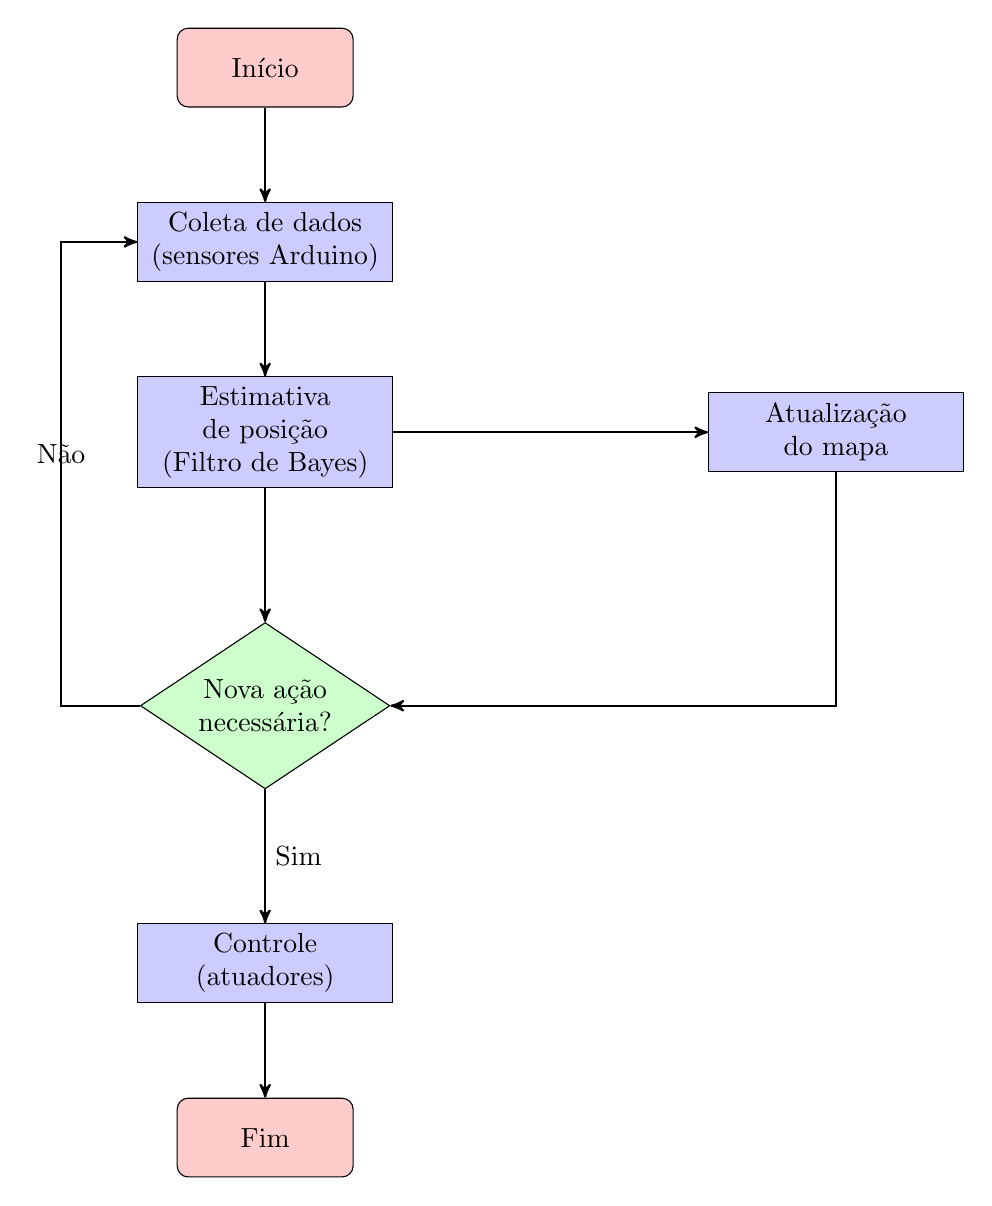
\begin{tikzpicture}[node distance=1.2cm and 1.5cm, auto]

% Estilos
\tikzset{
    startstop/.style={rectangle, rounded corners, draw, fill=red!20, text width=2cm, minimum height=1cm, text centered},
    process/.style={rectangle, draw, fill=blue!20, text width=3cm, minimum height=1cm, text centered},
    decision/.style={diamond, draw, fill=green!20, aspect=1.5, text width=2cm, inner sep=1pt, text centered},
    arrow/.style={->, >=stealth', thick}
}

% Nós
\node (start) [startstop] {Início};
\node (dataCollect) [process, below=of start] {Coleta de dados\\ (sensores Arduino)};
\node (localization) [process, below=of dataCollect] {Estimativa de posição\\ (Filtro de Bayes)};
\node (mapUpdate) [process, right=of localization, xshift=2.5cm] {Atualização do mapa};
\node (decision) [decision, below=of localization, yshift=-0.5cm] {Nova ação\\ necessária?};
\node (motion) [process, below=of decision, yshift=-0.5cm] {Controle\\ (atuadores)};
\node (stop) [startstop, below=of motion] {Fim};

% Setas
\draw [arrow] (start) -- (dataCollect);
\draw [arrow] (dataCollect) -- (localization);
\draw [arrow] (localization) -- (decision);
\draw [arrow] (localization) -- (mapUpdate);
\draw [arrow] (mapUpdate) |- (decision);
\draw [arrow] (decision) -- node[right] {Sim} (motion);
\draw [arrow] (decision.west) -- ++(-1,0) |- node[near start,above] {Não} (dataCollect.west);
\draw [arrow] (motion) -- (stop);

\end{tikzpicture}
    }
\end{frame}


\begin{frame}{Arquitetura de Processamento}
\centering
\scalebox{0.70}{
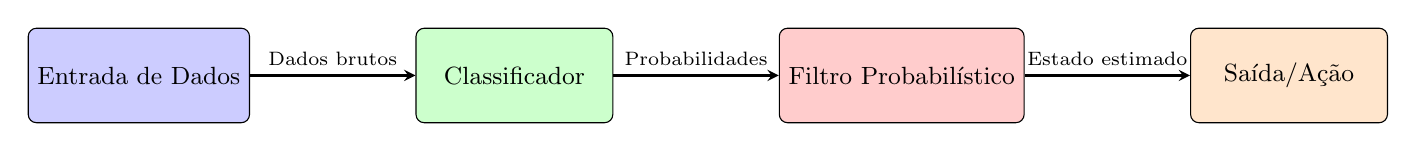
\begin{tikzpicture}[
    node distance=2.1cm,
    module/.style={
        rectangle, 
        draw, 
        rounded corners=3pt,
        minimum width=2.5cm, 
        minimum height=1.2cm,
        align=center, 
        font=\small,
        fill=#1!20
    },
    arrow/.style={->, >=stealth, thick}
]
    \node[module=blue] (input) {Entrada de Dados};
    \node[module=green, right=of input] (classifier) {Classificador};
    \node[module=red, right=of classifier] (filter) {Filtro Probabilístico};
    \node[module=orange, right=of filter] (output) {Saída/Ação};
    
    \draw[arrow] (input) -- node[above,font=\scriptsize] {Dados brutos} (classifier);
    \draw[arrow] (classifier) -- node[above,font=\scriptsize] {Probabilidades} (filter);
    \draw[arrow] (filter) -- node[above,font=\scriptsize] {Estado estimado} (output);
\end{tikzpicture}
}

\vspace{0.5cm}

\begin{columns}[T]
    \column{0.5\textwidth}
    \begin{block}{Classificador}
        \begin{itemize}
            \item Transforma dados brutos em informações semânticas
            \item Exemplos: 
                \begin{itemize}
                    \item Random Forest
                    \item Redes Neurais
                    \item SVM
                \end{itemize}
            \item Saída: Probabilidades ou categorias.
        \end{itemize}
    \end{block}
    
    \column{0.5\textwidth}
    \begin{block}{Filtro Probabilístico}
        \begin{itemize}
            \item Combina observações com conhecimento prévio
            \item Exemplos:
                \begin{itemize}
                    \item Filtro de Bayes
                    \item Filtro de Kalman
                    \item Filtro de Partículas
                \end{itemize}
            \item Saída: Estado estimado do sistema.
        \end{itemize}
    \end{block}
\end{columns}
\end{frame}

\begin{frame}
  \frametitle{Estrutura de um Robô}
  \begin{block}{Componentes Principais}
    \begin{itemize}
      \item Microcontroladores
      \item Sensores
      \item Atuadores
    \end{itemize}
  \end{block}
  
  \begin{center}
    \includegraphics[width=0.35\textwidth]{Image/arduino.jpg} % Imagem de um robô
    \vspace{0.2cm}
    
    % Fonte da imagem
    {\tiny \textbf{Fonte:} Ilustração gerada por OpenAI, 2024.}
  \end{center}
\end{frame}


% Diagrama de prototipagem com bordas arredondadas
\begin{frame}{Diagrama de Prototipagem}
    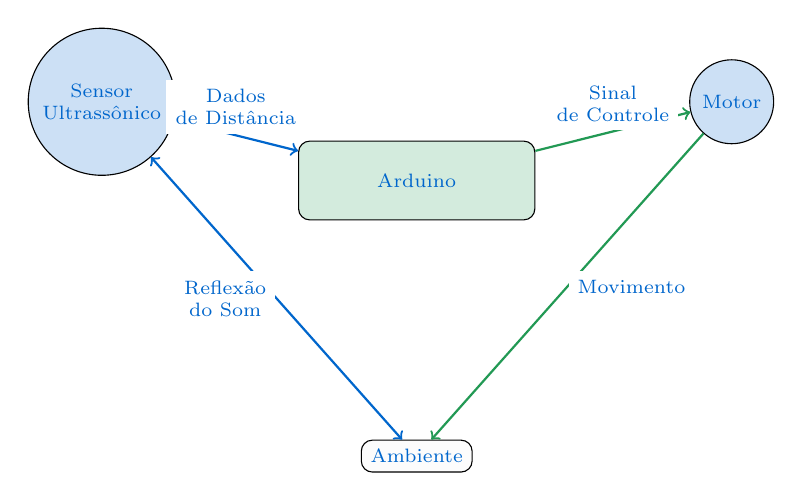
\begin{tikzpicture}[node distance=2.0cm, every node/.style={fill=white, font=\scriptsize, text=techblue}, align=center]
        \node (arduino) [rectangle, draw, rounded corners, fill=techgreen!20, minimum width=3cm, minimum height=1cm] {Arduino};
        \node (sensor) [circle, draw, fill=techblue!20, left of=arduino, xshift=-2cm, yshift=1cm] {Sensor\\Ultrassônico};
        \node (motor) [circle, draw, fill=techblue!20, right of=arduino, xshift=2cm, yshift=1cm] {Motor};
        \node (env) [rectangle, draw, rounded corners, fill=techgray!20, below of=arduino, yshift=-1.5cm] {Ambiente};
        \draw[->, thick, techblue] (sensor) -- (arduino) node[midway, above] {Dados\\de Distância};
        \draw[->, thick, techgreen] (arduino) -- (motor) node[midway, above] {Sinal\\de Controle};
        \draw[<->, thick, techblue] (env) -- (sensor) node[midway, left] {Reflexão\\do Som};
        \draw[->, thick, techgreen] (motor) -- (env) node[midway, right] {Movimento};
    \end{tikzpicture}
\end{frame}


%\begin{frame}{Aplicações de Robótica Probabilística na Questão Agrária}
%    \begin{itemize}
%        \item \textbf{Agricultura de Precisão}: Monitoramento eficiente do solo e das plantas, otimizando o uso de recursos.
%        \item \textbf{Detecção de Pragas e Doenças}: Identificação precoce com análise probabilística para controle direcionado.
%        \item \textbf{Navegação Autônoma}: Robôs mapeiam e navegam em terrenos agrícolas, reduzindo custos e mão-de-obra.
%        \item \textbf{Colheita Automatizada}: Identificação e colheita de frutos no ponto ideal usando visão computacional.
%        \item \textbf{Monitoramento Climático}: Coleta de dados ambientais para previsões e otimização da produção.
%    \end{itemize}
%\end{frame}
    
\section{Resultados Esperados}
\begin{frame}{Resultados Esperados}
    \begin{block}{Protótipos}
        \begin{itemize}
            \item Desenvolvimento de protótipos funcionais utilizando Arduino.
        \end{itemize}
    \end{block}
    \begin{block}{Modelagem}
        \begin{itemize}
            \item Análise da adaptação do robô a diferentes cenários com técnicas de programação estocástica.
        \end{itemize}
    \end{block}
    \begin{block}{Interação Robô-Ambiente}
        \begin{itemize}
            \item Investigação detalhada da interação entre o robô e o ambiente.
        \end{itemize}
    \end{block}

    \begin{block}{Autonomia e Robustez do Sistema}
        \begin{itemize} 
            \item Funcionamento autônomo em cenários dinâmicos com capacidade de adaptação a mudanças no ambiente.
        \end{itemize}
    
    \end{block}
\end{frame}

\begin{frame}{Publicações e Impacto}
    \begin{itemize}
        \item Elaboração da tese de doutorado com resultados da pesquisa.
        \item Publicações em revistas especializadas e apresentações em congressos.
        \item Contribuição significativa para o estudo em estatística computacional.
        \item Publicação de dois ou mais artigos em revistas especializas em Estatística aplicada ou Robótica.
    \end{itemize}
\end{frame}

\begin{frame}{Para publicação}
     \includegraphics[width=0.3\textwidth]{Image/journaEst.jpg} % Imagem de um robô
     \includegraphics[width=0.3\textwidth]{Image/journalRob.jpg} % Imagem de um robô
     %\includegraphics[width=0.3\textwidth]{Image/qciencia.png} % Imagem de um robô
    \vspace{0.2cm}
    
\end{frame}

\begin{frame}{Wiki do projeto}
    \begin{center}
        \qrcode[height=5cm]{https://github.com/Jeffreypir/ProbabiliticRobotics/wiki/Rob\%C3\%B3tica-Probabilistica}

          {\scriptfont  \textbf{Fonte:} Elaborado pelo autor.}
    \end{center}
\end{frame}

\section{Referências}
\section{Referências}
\begin{frame}{Referências}
    \footnotesize
    \begin{thebibliography}{99}
    
        \bibitem{cifuentes2019survey}
        CIFUENTES, Mario; SERRANO, Sergio. A survey of probabilistic algorithms for robotics. \textit{Journal of Robotics}, 2019.
        
        \bibitem{ross2014}
        ROSS, Sheldon M. \textit{Introduction to Probability Models}. Academic Press, 2014.

        \bibitem{Santos2024}
        SANTOS, Jefferson Bezerra dos. ProbabiliticRobotics. Disponível em: \url{https://github.com/Jeffreypir/ProbabiliticRobotics}. Acesso em: 13 set. 2024.

        \bibitem{siegmund2019introduction}
        SIEGMUND, Karl; HOFFMANN, Tilo. \textit{Introduction to Robotics: Analysis, Control, Applications}. CRC Press, 2019.
    
        \bibitem{smythe2021}
        SMYTHE, Richard J. \textit{Arduino Measurements in Science: Advanced Techniques and Data Projects}. New York: Apress, 2021.

        \bibitem{thrun2005probabilistic}
        THRUN, Sebastian; BURGARD, Wolfram; DURRANT-WHYTE, Hugh. \textit{Probabilistic Robotics}. MIT Press, 2005.

    \end{thebibliography}
\end{frame}
% \bibitem{barber2012bayesian}BARBER, David. \textit{Bayesian Reasoning and Machine Learning}. Cambridge University Press, 2012.
    
    \section{Agradecimentos}
\begin{frame}
    \frametitle{Agradeço a todos pela atenção!}
   % \begin{center}
   %     \begin{minipage}{0.1\textwidth} % Imagem à esquerda
          %  \includegraphics[width=\textwidth]{Image/logo.png}
   %     \end{minipage}%
   %     \hfill % Preenche o espaço entre os elementos
   %     \begin{minipage}{0.6\textwidth} % Texto centralizado
   %         \centering
          %  \textbf{Universidade Federal Rural de Pernambuco \\ Programa de Pós-Graduação em Biometria e Estatística Aplicada}
   %     \end{minipage}%
   %     \hfill % Preenche o espaço entre os elementos
   %     \begin{minipage}{0.1\textwidth} % Imagem à direita
   %         \includegraphics[width=\textwidth]{Image/PPGBEA.png}
   %     \end{minipage}
   % \end{center}

    \vspace{2cm} % Preenche o espaço entre os elementos
    \begin{minipage}{0.10\textwidth} % QR Code à esquerda da imagem de dúvida
        \qrcode{https://github.com/Jeffreypir/ProbabiliticRobotics/wiki/Rob\%C3\%B3tica-Probabilistica} 
        \centering
        \scalebox{0.9}{\tiny \hspace{0.3cm} Wiki do projeto}
    \end{minipage}%
    \vspace{-2cm}
    \begin{center}
        Perguntas?

        \begin{minipage}{0.35\textwidth} % Imagem de dúvida à direita do QR Code
            \includegraphics[width=\textwidth]{Image/duvida.png}
        \end{minipage}

        % Fonte da imagem
        {\tiny \textbf{Fonte:} Ilustração gerada por OpenAI, 2024.}
    \end{center}
\end{frame}
\end{document}

